%%%%
\section{África}

Os maiores níveis de poluição de ar no mundo ocorre
em cidades da ásia, oriente médio e áfrica \cite{brauer2012}.   

Embora a poluição do ar urbana em cidades nos países em 
desenvolvimento guarde algumas similaridades com as dos 
países desenvolvidos, como a poluição causada pelo tráfego, 
há ainda grandes diferenças, já que ainda é comum encontrar
a queima de biomassa como fonte de energia para cozimento em
cidades de países em desenvolvimento \cite{brauer2012}.

Assim, cidades de países africanos tem ganhado atenção em 
pesquisas sobre poluição e seus efeitos na sáude. 

%%%%
\subsection{África Subsariana}

A África Subsariana (SSA), localizada no norte da África, é atualmente 
a região no mundo que tem a maior taxa de transição da população rural 
- ainda predominante - para cidade \citep{MONTGOMERY2008}.

Mesmo assim, as cidades da \textit{SSA} ainda não possuem sistemas de 
monitoramento sistemático de poluição do ar e suas implicações na saúde 
\citep{EZZATI2004}. 
Além disso há poucas pesquisas acadêmicas dos níveis de poluição do ar nos 
países da \textit{SSA}.

Diferente dos países industrializado, onde as principais fontes de poluição 
são os setores da industria e do transporte, nos países da \textit{SSA} a 
queima de biomassa assume a primazia, sendo comum o seu uso no cozimento 
de alimentos, tanto em regiões urbanas quanto rurais \citep{SMITH2004}. 
Outras características regionais ampliam as diferenças na qualidade do ar 
e no perfil de fontes observado:

\begin{itemize}
  \item população predominantemente rural;
  \item muitas vias não pavimentadas;
  \item maior taxa de crescimento populacional urbano do mundo;
  \item não possuem sistemas de monitoramento sistemático de Poluição do Ar;
  \item é comum o uso da queima de biomassa para o cozimento de alimentos  
        (comercial e doméstico), tanto em regiões urbanas quanto rurais.
\end{itemize}


%%%%
\section{Gana}

Os últimos dois censos realizados em Gana datam
de 2000 \cite{censu2003} e 2010 \cite{censu2013}.

A população de gana em 2010 era de $24,7$ milhões, 
estando $49\%$ no meio rural e $61\%$ no meio urbano, 
sendo que as mulheres representam $51,2\%$ da polulação
total \cite{censu2013}.  

A população teve uma aumento de aproximadamente 
$30\%$ em 10 anos, já que era de $18,9$ milhões 
em 2000 \cite{censu2003}.

População ganense por faixa etária \ref{fig:piramedegana}. 

\begin{figure}[H]
\begin{center}
  \includegraphics[scale=0.4]{../outputs/piramide_etaria.pdf}
  \caption{Pirâmide etária Gana. Dados de \cite{censu2013} \label{fig:piramedegana}}
\end{center}
\end{figure}

A economia de Gana, antes essencialmente dominada pela agricultura, 
agora está distribuída entre: industria $19\%$, agricultura $30\%$ 
e serviços $51\%$ \cite{censu2013}. 

A responsabilidade do controle, fiscalização e monitoramento das 
atividades poluídoras em Gana é realizado pela 
\textbf{Ghana Environmental Protection Agency (EPA Ghana)} hierarquicamente
subordinada ao Ministério de Meio Ambiente, Ciência, Tecnologia e Inovação do 
governo federal de Gana.


%%%%
\section{Acra}

Acra é a capital de Gana e está localizada no Golfo Guiné. Ela tem uma área 
total de mais de 2500 $km^2$ com elevações que variam de 0 até 60 metros do nível 
do mar. é uma cidade litoranea;
%TODO: citar fonte 

A Região Metropolitana de Acra (RMA) agrega outras 9 cidades
além de Acra e conta com uma população de 4 milhões pessoas. 
Se caracteriza por ser essencialmente insdustrializada, com $90,5\%$ 
da polulação urbana \cite{censu2013}.

A densidade populacional em RMA é de 1205 $habitantes/km^2$, 
enquato que na Região Metropolitana de São Paulo (RMSP) é de 
2476 $habitantes/km^2$ \cite{ibge2011}. 

%TODO: acho que caberia ampliar as informações sobre Acra: 1) o que há sobre a frota veicular?; 2) quais são as atividades econômicas locais? 3) qual o PIB da cidade e de Ghana? 4) qual o PIB per capita?

\begin{table}[H]
 \centering
  \input{../outputs/census2010_cookfuel.tex}
  \caption{Fontes de energia usadas \cite{censu2013}}
\end{table}

Há aproximadamente 1000 fazendas urbanas com produção de vegetais em Acra e 
muitas delas usam água não tratada para irrigação. Altos indíces de 
metais pesados (Fe, Mn, Cu, Zn, Pb, Ni, Cr, Cd, Co)
foram encontrados nas plantações dessas fazendas \cite{lente2014} provindos 
principalmente de residências sem infraestrutura sanitária. 


\cite{asante2012} analisou nível de elementos traços nas urinas de trabalhadores 
do e-waste de Agbogbloshie e Fe, Sb, and Pb tiveram concentrações alta se comparada
a um pessoa de referência. 

Importação ilegal e reclicagem imprópria caracterizam Agbogbloshie.


% EPA GHANA
Fontes de poluição do ar ambinental mais importante em Acra:

- emissão veicular, principalmente emissões de veículos antigos sem manutenção
- Emissões industriais
- Queima de lixo e outros materiais a céu aberto
- poeira de solo
- vento seco harmatão


Compara com Brazil e WHO
Ambient Air Quality-EPA Ghana
NOx-24 hr (ug/m3) 150

PM10-24 hr (ug/m3) 70

SOx-24 hr ((ug/m3) 150

TSP-24 hr (ug/m3) 230
 November to March, which was the dry season.


os corregos de gana são feitos de  esgoto doméstico.


%%%%
\section{Nima}

\begin{figure}[H]
  \caption{Fotos do bairro de Nima}
  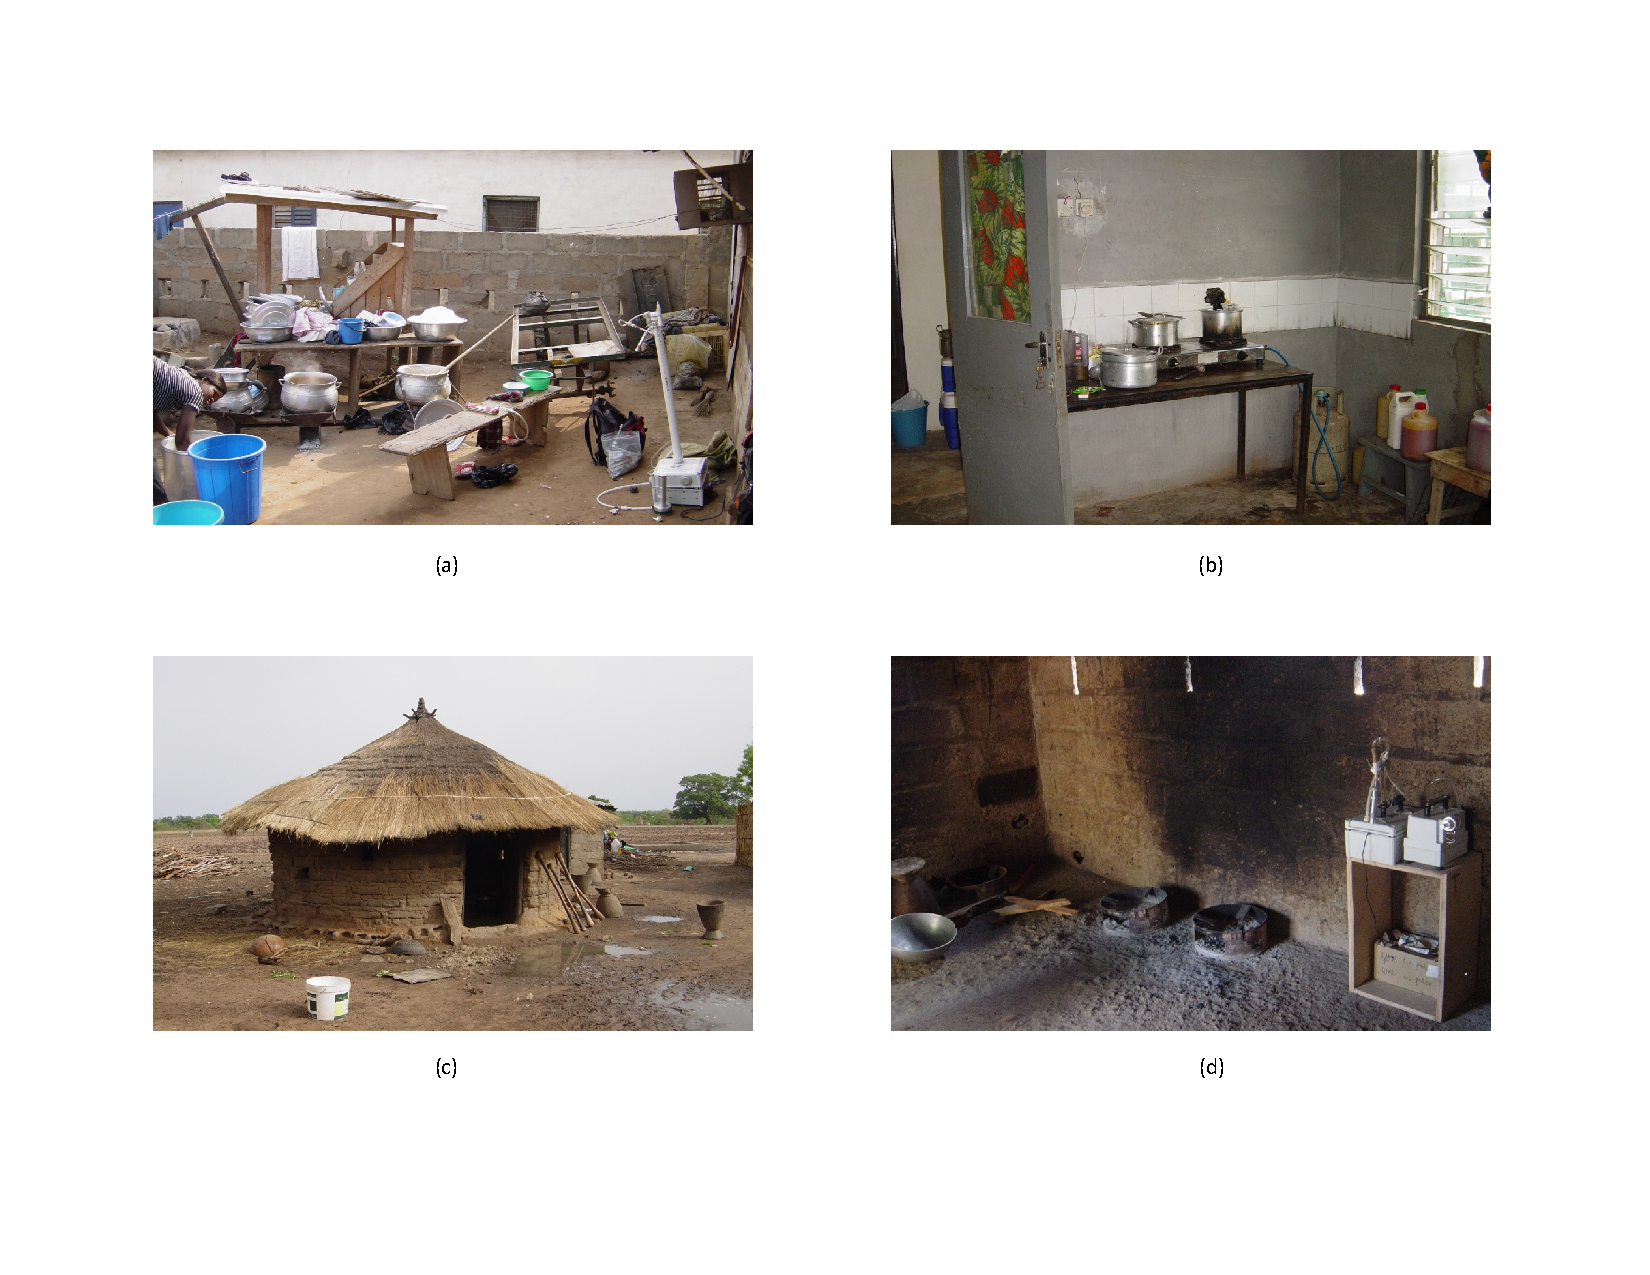
\includegraphics[scale=0.35]{../inputs/images/zheng/nima.pdf}
\end{figure}

%TODO: acho que essas fotos são de Nima e de uma zona rural. É importante ter um mapa que localize Ghana, destaque Acra e neste último destaque Nima. Quais as características deste bairro? Qual o contraste com os demais?

\begin{figure}[H]
\begin{center}
  \includegraphics[width=0.9\textwidth]{../outputs/accra_sources.pdf}
  \caption{sources}
\end{center}
\end{figure}

disposição geográfica dos principais poluidores atmosféricos
Na figura estão assinalados a estação de medida e e um conjunto de fontes emissoras 
de grande porte operando na RMR ou em seu entorno, bem como as estações 
meteorológicas do aeroporto.


%%%%
\section{Projeto Internacional}

Este trabalho enquadra-se no projeto de pesquisa internacional 
\textit{Air Pollution in Accra Neighborhoods: Spatial, Socioeconomic, and Temporal Patterns} 
coordenado por pesquisadores da \textit{Harvard School of Public Health} nos Estados Unidos, 
com participação da Universidade de Ghana. 
Coordenado pelo Dr Majid Ezzati, a época professor da \textit{Harvard School of Public Health} 
nos Estados Unidos (atualmente no Imperial College London, na Inglaterra), com participação 
da Universidade de Ghana. 

A interação entre grupos de pesquisa de diferente áreas como, saúde, estatística,
medicina e aqueles capazes de quantificar, analisar processos e 
identificar fontes geradoras de poluentes é fundamental

Os países da \textit{África Subsariana (SSA)} possuem a maior taxa de crescimento 
populacional urbano do mundo \cite{united2006world}, mas ainda possuem uma população 
predominantemente rural. 
Apesar disso, ainda é escasso o conhecimento do impacto que esse novo modelo de vida 
tem causado para saúde e meio ambiente na SSA \cite{cohen2004urban}. 

Pioneiro nas pesquisas de poluição do ar ambiental em países da SSA, o objetivo 
global desse projeto internacional é fazer avaliações iniciais e sistemáticas 
dos níveis de poluição do ar em Acra (capital de Gana e maior cidade da SSA), 
inexistentes até então, e relacioná-los com as condições socioeconômicas 
específicas das diferentes áreas estudadas naquela capital.

Poucos estudos sobre poluição atmosférica foram realizados em \textbf{Gana}, 
sendo \citep{ARKU2008} e \citep{DIONISIO2010} pioneiros em conduzirem 
levantamento nos níveis de poluição, composição elementar e distribuição espacial 
e temporal de poluentes. 



